\chapter{The LVish Library: Implementation and Evaluation\label{ch:lvish}} % 4

\TODO{Revise this chapter.}

\lk{What follows is from the FHPC paper and needs to be edited or removed.}

\section{Prototype Implementation and Evaluation}\label{section:evaluation}

We have implemented a prototype LVars library based on
the {\em monad-par} Haskell library, which provides the @Par@ monad \cite{monad-par}.
Our library, together with example programs and preliminary
benchmarking results, is available in in the LVars repository.
{The relationship to $\lambdaLVar$ is somewhat loose: for instance,
  while evaluation in $\lambdaLVar$ is always strict, our library allows
  lazy, pure Haskell computations along with strict, parallel monadic computations.}

%\footnote{Not literally, but as System F underpins Haskell.}.

%% If we could use arbitrary monotonic data structures, then multiple threads could
%% traverse the connected component, adding node-labels to a {\em set}, with the
%% function $F$ computed over each label in that growing set.  For example, the following
%% program implements a {\em level-synchronized} BFS in this way:

\begin{figure}
  \lstinputlisting{chapter2/code/bfs_lvar.hs}
  \caption{\footnotesize 
    An example Haskell program, written using our LVars library, that
    maps a computation over a connected component using a monotonically
    growing set variable.  The code is written in a strict style, using the \lstinline|Par|
    monad for parallelism.  The use of the set variable enables modularity and
    safe pipelining.  Consumers can safely asynchronously execute work items
    put into \lstinline|analyzedSet|.}
  \label{f:bfs-lvar}
\end{figure}

%% \lk{I think that one point that is missing from this section and needs
%%   to be made is how LVars compare with IVars for the purpose of
%%   writing programs like this.  Sure, we know that we can't use IVars
%%   for mark bits, but we obviously didn't end up needing to use mark
%%   bits anyway -- so, what have we really done here that we couldn't
%%   have done (as easily) with IVars?}
%% \rn{I put this in below, it's also hopefully now more obvious above.}


%\begin{figure*}[tb]
\begin{figure*}
 \centering 
%  \includegraphics[clip,trim=200px 200px 300px 200px,width=2.3in]{figures/BFS.pdf} 
%  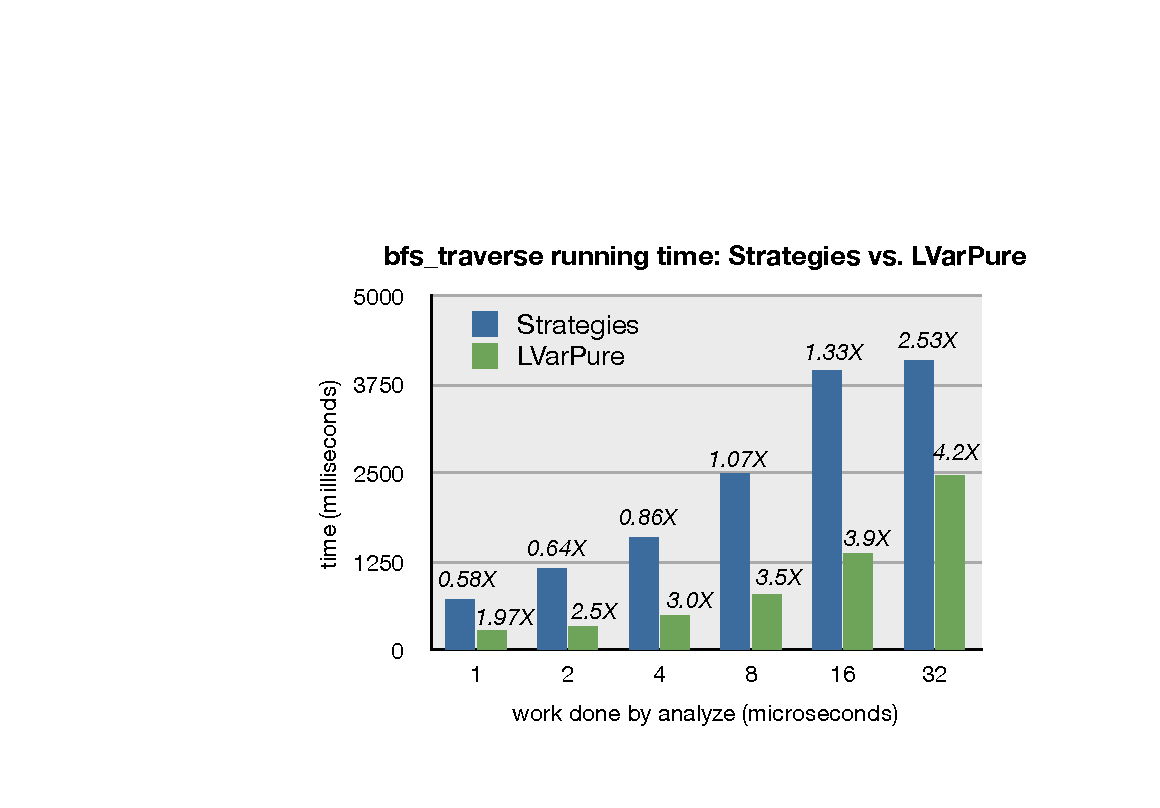
\includegraphics[width=2.5in]{figures/bargraph_with_speedups2.pdf} 
%  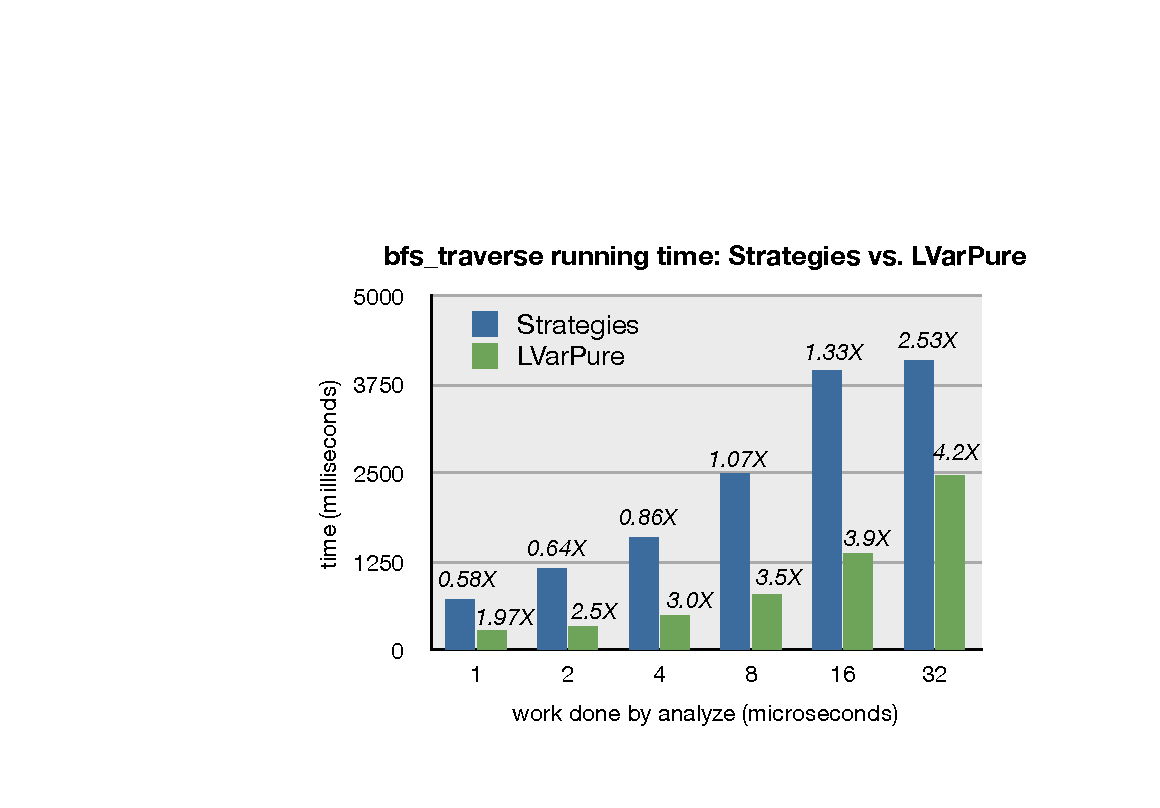
\includegraphics[width=2.7in]{figures/bargraph_with_speedups2.pdf} 

% . . side top
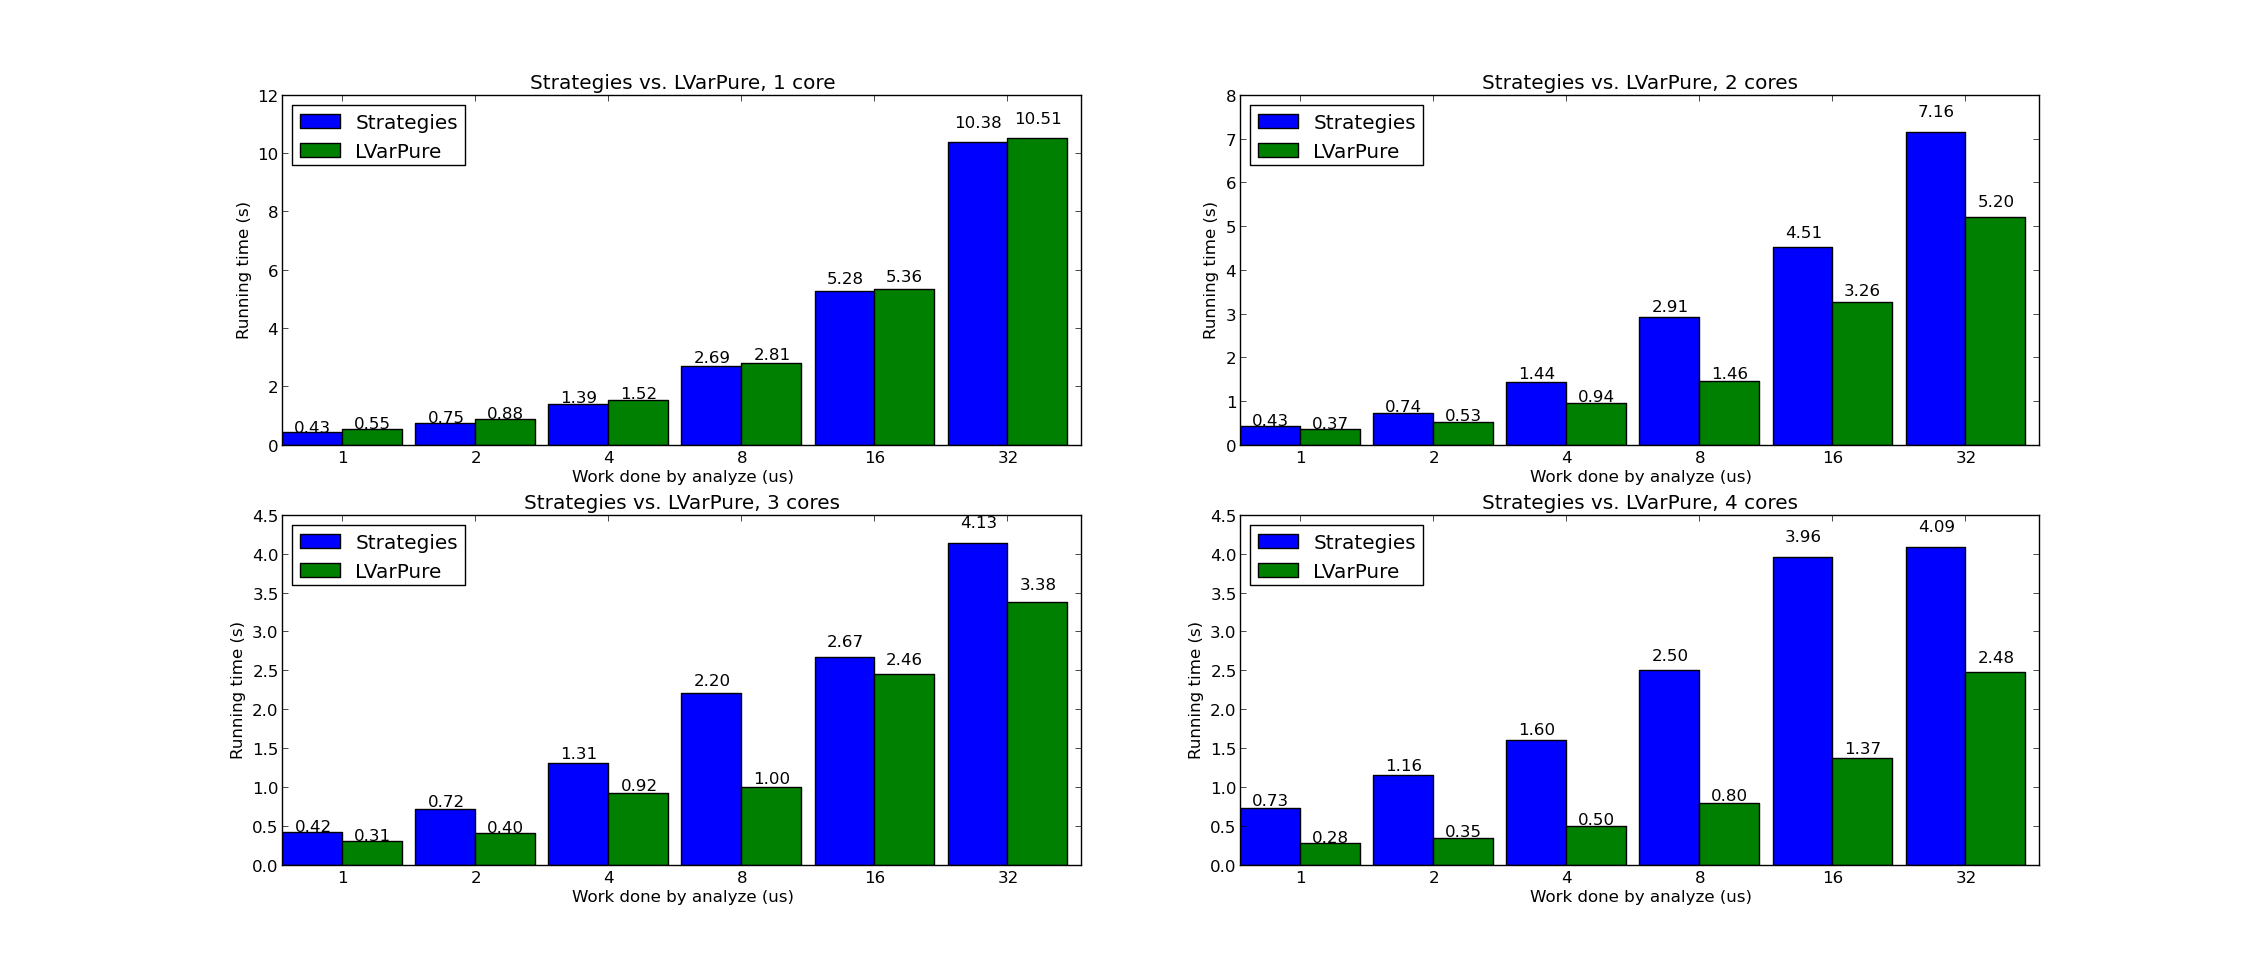
\includegraphics[clip, trim=150px 0px 0px 35px, width=7.8in, natwidth=2266px, natheight=962px]{chapter2/figures/bf_traverse_benchmark_data.png} 
\vspace{-8mm}
  \caption{\footnotesize Running time comparison of Strategies-based and LVar-based
    implementations of \lstinline|bf_traverse|, running on 1, 2, 3, and 4 cores on
    an Intel Xeon Core i5 3.1GHz (smaller is better).}
  %% \caption{\footnotesize Running time comparison of Strategies and of LVar-based
  %%   implementations of \lstinline|bf_traverse|, running on 4 cores on
  %%   an Intel Xeon Core i5 3.1GHz.  Smaller is better; numbers at top of bars indicate
  %%   parallel speedup relative to serial version of the same algorithm.}
  \label{f:performance}
\end{figure*}

%\subsection{Implementations}
\paragraph{A layered implementation}

%% \new{There are {\em three} relevant parties in deploying LVars: the 
%%   runtime implementor, the data structure author who provides an
%%   implementation for a specific lattice (\eg, a monotonically growing hashmap),
%%   and the application writer who uses LVars.  Only the application writer receives
%%   a determinism guarantee.  The data structure author uses
%%   an interface provided by the runtime implementor, who provides core functionality:
%%   thread scheduling and tracking of threads blocked on $\GET$ operations.
%% }

Use of our LVars library typically involves two parties: first, the data
structure author who uses the library directly and provides an
implementation of a specific monotonic data structure (\eg, a
monotonically growing hashmap), and, second, the application writer
who uses that data structure.  Only the application writer receives a
determinism guarantee; it is the data structure author's obligation to ensure
that the states of their data structure form a lattice and that it is only accessible via
the equivalent of $\PUT$ and $\GET$.

The data structure author uses an interface provided by our LVars library,
which provides core runtime functionality: thread scheduling and
tracking of threads blocked on $\GET$ operations.
%% We provide three implementations of our LVar library, each of which can be instantiated
%% with any lattice(s).  All three 
Concretely, 
the data structure author
imports our library
and reexports a limited interface specific to their data structure 
(\eg{}, for sets, @putInSet@ and @waitSetSizeThreshold@).  
%% Again, it is important that entire LVar runtime interface 
%% {\em not} be exported to end users of the data-structure library,
%% because if the states of the data structure do not satisfy
%% the properties of a lattice, things can go awry.  
\new{In fact, our library provides three different runtime interfaces for the data structure author
to choose among.  These ``layered'' interfaces provide the data structure author with a shifting
trade-off between the {\em ease} of meeting their proof obligation, and {\em attainable performance}:}

\begin{enumerate}
\item {\bf Pure LVars}: Here, each LVar is a single mutable
  container (an @IORef@) containing a pure value.  This requires only
  that a library writer select a purely functional data structure and
  provide a @join@\footnote{Type class
    \lstinline|Algebra.Lattice.JoinSemiLattice|.} function for it and a threshold
  predicate for each @get@ operation.  These pure functions are
  easiest to validate, for example, using the popular QuickCheck \cite{quickcheck} tool.

\item {\bf IO LVars}: Pure data structures in mutable containers
  cannot always provide the best performance for concurrent data
  structures.
% \cite{my-haskell-implementors-talk-if-there-is-space}.
  Thus we provide a more effectful interface.  With it, data
  structures are represented in terms of arbitrary mutable state; performing a
  @put@ requires an {\em update action} (@IO@) and a @get@ requires an
  effectful polling function that will be run after any @put@ to the
  LVar, to determine if the @get@ can unblock.

\item {\bf Scalable LVars}: Polling each blocked @get@ upon {\em any}
  @put@ is not very precise.  If the data structure author takes on yet more
  responsibility, they can use our third interface to reduce contention by
  managing
   the storage of blocked computations and threshold functions {\em
     themselves}.  
  For example, a concurrent set
  might store a waitlist of blocked continuations on a per-element basis,
  rather than using one waitlist for the entire LVar, as in layers (1) and (2).
\end{enumerate}

\noindent The support provided to the data structure author {\em declines} with each of
these layers, with the final option providing only parallel scheduling,
and little help with defining the specific LVar data structure.  But
this progressive cost/benefit tradeoff can be beneficial for
prototyping and then refining data structure implementations.  

% \begin{lst}
% putLV :: LVar a -> (a -> IO ()) -> Par ()
% getLV :: LVar a -> (IO (Maybe b)) -> Par b

% pure
% getLV :: LVar a -> (a -> Maybe b) -> Par b
% putLV :: JoinSemiLattice a => LVar a -> a -> Par ()

\paragraph{Revisiting our breadth-first traversal example}

In Section~\ref{section:motivation}, we proposed using LVars to
implement a program that performs a breadth-first traversal of a
connected component of a graph, mapping a function over each node in
the component.
Figure~\ref{f:bfs-lvar} gives a version of this program implemented using our LVars library.
It performs a breadth-first traversal of the 
 @profiles@ graph with effectful $\PUT$
operations on a shared set variable.  
\new{This variable, \lstinline|analyzedSet|, has to be modified
multiple times by \lstinline|putInSet| and thus cannot be an IVar.\footnote{Indeed, there are
  subtle problems with encoding a set even as a linked structure of
  IVars.  For example, if it is represented as a tree, who writes the root?}  The callback function
 \lstinline|analyze| is ``baked into'' \lstinline|analyzedSet| and may run
  as soon as new elements are inserted.  
  %% (In the $\lambdaLVar$ calculus,
  %% \lstinline|analyze| could be built into the $\REIFY$ function
  %% and applied to the result of $\GET$.)
}
Our implementation uses the ``Pure LVars'' runtime layer described above: 
@analyzedSet@ is nothing more than a tree-based data structure
(@Data.Set@) stored in a mutable location.  

\paragraph{Preliminary benchmarking results}

We compared the performance of the LVar-based implementation of @bf_traverse@ against the version in Figure~\ref{f:bfs-pure}, which we ran using the 
\\ @Control.Parallel.Strategies@ library
\cite{marlow-par}, version 3.2.0.3. (\new{Despite being a simple algorithm, even breadth-first search by itself
is considered a useful benchmark; in fact, the well-known
``Graph 500'' \cite{graph500} benchmark is exactly breadth-first search.})

We evaluated the Strategies and LVar versions of @bf_traverse@
by running both on a local random directed graph of 40,000 nodes and
320,000 edges (and therefore an average degree of 8), simulating the
@analyze@ function by doing a specified amount of work for each node,
which we varied from 1 to 32 microseconds.
Figure \ref{f:performance} shows the results of our evaluation on 1, 2, 3, and 4 cores.
Although both the Strategies and LVar versions enjoyed a
 speedup as we added parallel resources, the LVar
version scaled particularly well.
A subtler, but interesting point is that, in the Strategies version,
it took an average of 64.64 milliseconds for the first invocation of
@analyze@ to begin running after the program began, whereas in the
LVar version, it took an average of only 0.18 milliseconds,
indicating that the LVar version allows work to be
pipelined.



\rnote{Report time-to-first-f results in prose I suppose....}


%% \lk{Shouldn't stuff like this be pushed to an evaluation section
%%   further along in the paper?  Not sure it belongs right in the
%%   intro.}
%% \new{In fact, we know it is possible to implement these data structures even more
%% efficiently.  The key question addressed in this paper, is not whether
%% such a system can be implemented, but:}
%The question then becomes: 
%% {\em how might we convince ourselves that every program
%% written with such a library is deterministic, especially when mixing different
%% data structures?}
%% \rn{TODO: More explicitly declare here that the paper is not about this
%%   implementation, but about the underlying theory.}
%
%% The existence of, and usefulness of, practical implementations motivates
%% us to pursue this question.




\lk{What follows is from the POPL paper and needs to be edited.}

Our library comes with a number of monotonic data structures,
including sets, maps, counters, and single-assignment variables.
Further, it can be extended with new data structures, all of which can
be used compositionally within the same program.  Adding a new data
structure typically involves porting an existing scalable (\eg, {\em
  lock-free}) data structure to Haskell, then wrapping it to expose a
(quasi-)deterministic LVar interface.  Our library exposes a monad
that is \emph{indexed} by a determinism level: fully deterministic or
quasi-deterministic.  Thus, the \emph{static type} of an LVish
computation reflects its guarantee, and in particular the freeze-last
idiom allows freezing
 
In Section~\ref{section:eval}, we evaluate our library with a case
study: parallelizing control flow analysis.  The case study begins
with an existing implementation of $k$-CFA~\cite{MightkCFABlog}
written in a purely functional style.  We show how this code can
easily and safely be parallelized by adapting it to the LVish
model---an adaptation that yields promising parallel speedup, and also
turns out to have benefits even in the sequential case.

\section{Implementation}\label{section:implementation}

%Benefits of Haskell: monads + phantom types 

We have constructed a prototype implementation of LVish as a monadic library in
Haskell, which is available at 
\begin{center}
\url{http://hackage.haskell.org/package/lvish}
\end{center}
\ajt{Or would we rather link to github?}%
Our library adopts the basic approach
of the @Par@ monad~\cite{monad-par}, enabling us to employ our own notion of
lightweight, library-level threads with a custom scheduler.  It supports the
programming model laid out in Section~\ref{section:lvish-informal} in full,
including explicit handler pools.  It differs from our formal model in following
Haskell's by-need evaluation strategy, which also means that concurrency in the
library is \emph{explicitly marked}, either through uses of a @fork@ function or
through asynchronous callbacks, which run in their own lightweight thread.

Implementing LVish as a Haskell library makes it possible to provide
compile-time guarantees about determinism and quasi-determinism,
because programs written using our library run in our @Par@ monad and
can therefore only perform LVish-sanctioned side effects.
We take advantage of
this fact by indexing @Par@ computations with a phantom type
that indicates their \emph{determinism level}:
\begin{lstlisting}
  data Determinism = Det | QuasiDet
\end{lstlisting}
%% while the second is the standard phantom type used by the @ST@ monad, which is
%% used to ensure that LVars themselves cannot escape from uses of our @Par@ monad.
The @Par@ type constructor has the following kind:\footnote{We are here using
  the {\tt DataKinds} extension to Haskell to treat {\tt Determinism} as a
  kind.  In the full implementation, we include a second phantom type parameter to ensure that LVars
  cannot be used in multiple runs of the {\tt Par} monad, in a manner analogous to how the {\tt ST} monad prevents an {\tt STRef} from being returned from {\tt runST}.}
\begin{lstlisting}
  Par :: Determinism -> * -> *
\end{lstlisting}
together with the following suite of @run@ functions:
\begin{lstlisting}
  runPar   :: Par Det a -> a
  runParIO :: Par lvl a -> IO a
  runParThenFreeze :: DeepFrz a => Par Det a -> FrzType a
\end{lstlisting}
The public library API ensures that if code uses @freeze@, it is marked as
@QuasiDet@; thus, code that types as @Det@ is guaranteed to be fully
deterministic.  While LVish code with an arbitrary determinism level @lvl@ can be
executed in the @IO@ monad using @runParIO@, only @Det@ code can be executed as if it were pure,
since it is guaranteed to be free of visible side effects of nondeterminism.  In
the common case that @freeze@ is only needed at the end of an
otherwise-deterministic computation, @runParThenFreeze@ runs the computation to
completion, and then freezes the returned LVar, returning its exact value---and
is guaranteed to be deterministic.\footnote{The {\tt DeepFrz} typeclass is used
  to perform freezing of nested LVars, producing values of frozen type (as given
  by the {\tt FrzType} type function).}

%% The type @s@ (short for ``session'') that
%% appears in the @run@ functions also appears as a phantom type of LVars
%% themselves; the universal quantification forces each LVar to be tied to a single
%% session, \ie, a single use of a @run@ function~\cite{?}.  Readers unfamiliar with this
%% trick from the @ST@ monad can safely ignore the type parameter altogether.

\ajt{We don't actually prove that freeze-free code is deterministic, but it
  should follow pretty easily from the proof of quasi-determinism.  Perhaps we
  should claim it in the proof section?}
\lk{Well, to do this ``right'' we would have to not just prove that
  freeze-free code is deterministic, but we'd have to prove that
  freeze-happens-last code is deterministic...}

\subsection{The Big Picture}

We envision two parties interacting with our library.  First, there are data
structure authors, who use the library directly to implement a specific
monotonic data structure (\eg, a monotonically growing finite map).  Second,
there are application writers, who are clients of these data structures.  Only
the application writers receive a \mbox{(quasi-)determinism} guarantee; an author of a
data structure is responsible for ensuring that the states their data structure can take on
correspond to the elements of a lattice, and that the exposed interface to it corresponds to
some use of @put@, @get@, @freeze@, and event handlers.

Thus, our library is focused primarily on \emph{lattice-generic} infrastructure:
the @Par@ monad itself, a thread scheduler, support for blocking and signaling
threads, handler pools, and event handlers.  Since this infrastructure is unsafe
(does not guarantee quasi-determinism), only data structure authors should
import it, subsequently exporting a \emph{limited} interface specific to their
data structure.  For finite maps, for instance, this interface might include key/value
insertion, lookup, event handlers and pools, and freezing---along with
higher-level abstractions built on top of these.

For this approach to scale well with available parallel resources, it is
essential that the data structures themselves support efficient parallel access;
a finite map that was simply protected by a global lock would force all parallel
threads to sequentialize their access.  Thus, we expect data structure authors
to draw from the extensive literature on scalable parallel data structures,
employing techniques like fine-grained locking and lock-free data
structures~\cite{art}.  Data structures that fit into the LVish model have a
special advantage: because all updates must commute, it may be possible to avoid
the expensive synchronization which \emph{must} be used for non-commutative
operations~\cite{lawsOfOrder}.  And in any case, monotonic data structures are usually
much simpler to represent and implement than general ones.

\subsection{Two Key Ideas}\label{subsection:atomic}

%Our implementation strategy relies on two semantic observations:

\paragraph{Leveraging atoms}

Monotonic data structures acquire ``pieces of
information'' over time.  In a lattice, the smallest such pieces are called the
\emph{atoms} of the lattice: they are elements not equal to $\bot$, but for
which the only smaller element is $\bot$.  Lattices for which every element is
the lub of some set of atoms are called \emph{atomistic}, and in practice most
application-specific lattices used by LVish programs 
have this property---especially those whose elements represent
collections.

In general, the LVish primitives allow arbitrarily large queries and updates
to an LVar.  But for an atomistic lattice, the corresponding data structure
usually exposes operations that work at the atom level, semantically limiting
@put@s to atoms, @get@s to threshold sets of atoms, and event sets to sets of
atoms.  For example, the lattice of finite maps is atomistic, with atoms
consisting of all singleton maps (\ie, all key/value pairs).  The interface to a
finite map usually works at the atom level, allowing addition of a new
key/value pair, querying of a single key, or traversals (which we model as
handlers) that walk over one key/value pair at a time.

Our implementation is designed to facilitate good performance for atomistic
lattices by associating LVars with a set of \emph{deltas} (changes), as well as
a lattice.  For atomistic lattices, the deltas are essentially just the
atoms---for a set lattice, a delta is an element; for a map, a key/value pair.
Deltas provide a compact way to represent a change to the lattice, allowing us
to easily and efficiently communicate such changes between @put@s and
@gets@/handlers.

\paragraph{Leveraging idempotence}

While we have emphasized the commutativity of least upper bounds, they also
provide another important property: \emph{idempotence}, meaning that
$\userlub{d}{d} = d$ for any element $d$.  In LVish terms, repeated @put@s or @freeze@s
have no effect, and since these are the only way to modify the store, the
result is that $e; e$ behaves the same as $e$ for any LVish expression $e$.  
Idempotence has already been recognized as a useful property for work-stealing
scheduling~\cite{idempotent}: if the scheduler is allowed to occasionally duplicate work, it is
possible to substantially save on synchronization costs.  Since LVish
computations are guaranteed to be idempotent, we could use such a scheduler
(for now we use the standard Chase-Lev deque~\cite{ChaseLev}).  But idempotence
also helps us deal with races between @put@ and @get@/@addHandler@, as we explain below.
%%   Since
%% @addHandler@ must launch callbacks for any events that have already occurred, it
%% will must perform a traversal of the data structure; if that traversal is
%% concurrent with a @put@, the added data may or may not be seen

\subsection{Representation Choices}
Our library uses the following generic representation for LVars:
\begin{lstlisting}
  data LVar a d = 
       LVar { state :: a,  status :: IORef (Status d) }
\end{lstlisting}
where the type parameter @a@ is the (mutable) data structure representing the
lattice, and @d@ is the type of deltas for the lattice.\footnote{For
  non-atomistic lattices, we take \termfont{a} and \termfont{d} to be the same type.}
The @status@ field is a mutable reference that represents the status bit:
\begin{lstlisting}
  data Status d = Frozen | Active (B.Bag (Listener d))
\end{lstlisting}
The status bit of an LVar is tied together with a bag of waiting
\emph{listeners}, which include blocked @get@s and handlers; once the LVar is
frozen, there can be no further events to listen for.\footnote{In particular,
  with one atomic update of the flag we both mark the LVar as frozen and allow
  the bag to be garbage-collected.}  The bag module (imported as @B@) supports
atomic insertion and removal, and \emph{concurrent} traversal:
\begin{lstlisting}
  put     :: Bag a -> a -> IO (Token a)
  remove  :: Token a -> IO ()
  foreach :: Bag a -> (a -> Token a -> IO ()) -> IO ()
\end{lstlisting}
Removal of elements is done via abstract \emph{tokens}, which are acquired by
insertion or traversal.  Updates may occur concurrently with a traversal, but
are not guaranteed to be visible to it.
%which allows the entire bag to become garbage immediately after freezing.

A listener for an LVar is a pair of callbacks,
one called when the LVar's lattice value changes,
 and the other when the LVar is frozen:  
\begin{lstlisting}
 data Listener d = Listener {
   onUpd :: d -> Token (Listener d) -> SchedQ -> IO (),
   onFrz ::      Token (Listener d) -> SchedQ -> IO () }
\end{lstlisting}
The listener is given access to its own token in the listener bag, which it can
use to deregister from future events (useful for a @get@ whose threshold has
been passed).  It is also given access to the CPU-local scheduler queue, which
it can use to spawn threads.

\subsection{The Core Implementation}

Internally, the @Par@ monad represents computations in continuation-passing
style, in terms of their interpretation in the @IO@ monad:
\begin{lstlisting}
  type ClosedPar = SchedQ -> IO ()
  type ParCont a = a -> ClosedPar
  mkPar :: (ParCont a -> ClosedPar) -> Par lvl a
\end{lstlisting}
The @ClosedPar@ type represents ready-to-run @Par@ computations, which are given
direct access to the CPU-local scheduler queue.  Rather than returning a final
result, a completed @ClosedPar@ computation must call the scheduler, @sched@, on
the queue.  A @Par@ computation, on the other hand, completes by passing its
intended result to its continuation---yielding a @ClosedPar@ computation.

Figure~\ref{fig:implementation} gives the implementation for three core
lattice-generic functions: @getLV@, @putLV@, and @freezeLV@, which we explain next.

\begin{figure}
\lstset{basicstyle=\footnotesize\ttfamily}
\begin{lstlisting}
getLV :: (LVar a d) -> (a -> Bool -> IO (Maybe b)) 
                    -> (d -> IO (Maybe b)) -> Par lvl b
getLV (LVar{state, status}) gThresh dThresh = 
  mkPar $\k q -> 
    let onUpd d = unblockWhen (dThresh d)
        onFrz   = unblockWhen (gThresh state True)
        unblockWhen thresh tok q = do
          tripped <- thresh
          whenJust tripped $ \b -> do
            B.remove tok
            Sched.pushWork q (k b)                     
    in do
      curStat <- readIORef status
      case curStat of
        Frozen -> do   -- no further deltas can arrive!
          tripped <- gThresh state True
          case tripped of
            Just b  -> exec (k b) q
            Nothing -> sched q     
        Active ls -> do
          tok <- B.put ls (Listener onUpd onFrz)
          frz <- isFrozen status -- must recheck after
                                 -- enrolling listener
          tripped <- gThresh state frz
          case tripped of
            Just b  -> do
              B.remove tok  -- remove the listener 
              k b q         -- execute our continuation
            Nothing -> sched q

putLV :: LVar a d -> (a -> IO (Maybe d)) -> Par lvl ()
putLV (LVar{state, status}) doPut = mkPar $ \k q -> do  
  Sched.mark q  -- publish our intent to modify the LVar
  delta   <- doPut state      -- possibly modify LVar
  curStat <- readIORef status -- read while q is marked
  Sched.clearMark q           -- retract our intent
  whenJust delta $ \d -> do
    case curStat of
      Frozen -> error "Attempt to change a frozen LVar"
      Active listeners -> B.foreach listeners $ 
        \(Listener onUpd _) tok -> onUpd d tok q
  k () q 

freezeLV :: LVar a d -> Par QuasiDet ()
freezeLV (LVar {status}) = mkPar $ \k q -> do
  Sched.awaitClear q
  oldStat <- atomicModifyIORef status $ \s->(Frozen, s)    
  case oldStat of
    Frozen -> return ()
    Active listeners -> B.foreach listeners $ 
      \(Listener _ onFrz) tok -> onFrz tok q
  k () q
\end{lstlisting}
\caption{Implementation of key lattice-generic functions.}\label{fig:implementation}
%\vspace{-7mm}
\end{figure}

\paragraph{Threshold reading}

The @getLV@ function assists data structure authors in writing operations with
@get@ semantics.  In addition to an LVar, it takes two \emph{threshold
  functions}, one for global state and one for deltas.  The \emph{global threshold} @gThresh@ is
used to initially check whether the LVar is above some lattice value(s) by
global inspection; the extra boolean argument gives the frozen status of the
LVar.  The \emph{delta threshold} @dThresh@ checks whether a particular update 
takes the state of the LVar above some lattice state(s).
Both functions return @Just r@ if the threshold
has been passed, where @r@ is the result of the read.
To continue our running example of finite maps with
key/value pair deltas, we can use @getLV@ internally to build the following
@getKey@ function that is exposed to application writers:
\begin{lstlisting}
  -- Wait for the map to contain a key; return its value
  getKey key mapLV = getLV mapLV gThresh dThresh where
    gThresh m frozen = lookup key m
    dThresh (k,v) | k == key  = return (Just v)
                  | otherwise = return Nothing 
\end{lstlisting}
where @lookup@ imperatively looks up a key in the underlying map.

The challenge in implementing @getLV@ is the possibility that a
\emph{concurrent} @put@ will push the LVar over the threshold.  To cope with
such races, @getLV@ employs a somewhat pessimistic strategy: before doing
anything else, it enrolls a listener on the LVar that will be triggered on any
subsequent updates.  If an update passes the delta threshold, the listener is
removed, and the continuation of the @get@ is invoked, with the result, in a new
lightweight thread.  \emph{After} enrolling the listener, @getLV@ checks the
\emph{global} threshold, in case the LVar is already above the threshold.  If it
is, the listener is removed, and the continuation is launched immediately;
otherwise, @getLV@ invokes the scheduler, effectively treating its continuation
as a blocked thread.  

By doing the global check only after enrolling a listener, @getLV@ is sure not
to miss any threshold-passing updates.  It does \emph{not} need to synchronize
between the delta and global thresholds: if the threshold is passed just as
@getLV@ runs, it might launch the continuation twice (once via the global check,
once via delta), but by idempotence this does no harm.  This is a performance
tradeoff: we avoid imposing extra synchronization on \emph{all} uses of @getLV@
at the cost of some duplicated work in a rare case.  We can easily provide a
second version of @getLV@ that makes the alternative tradeoff, but as we will
see below, idempotence plays an \emph{essential} role in the analogous situation
for handlers.

\paragraph{Putting and freezing}

On the other hand, we have the @putLV@ function, used to build operations with
@put@ semantics.  It takes an LVar and an \emph{update function} @doPut@ that
performs the @put@ on the underlying data structure, returning a delta if the
@put@ actually changed the data structure.  If there is such a delta, @putLV@
subsequently invokes all currently-enrolled listeners on it.

The implementation of @putLV@ is complicated by another race, this time with
freezing.  If the @put@ is nontrivial (\ie, it changes the value of the LVar), the
race can be resolved in two ways.  Either the freeze takes effect first, in
which case the @put@ must fault, or else the @put@ takes effect first, in which case
both succeed.  Unfortunately, we have no means to both check the frozen status
\emph{and} attempt an update in a single atomic step.\footnote{While we could
  require the underlying data structure to support such transactions, doing so
  would preclude the use of existing lock-free data structures, which tend to
  use a single-word compare-and-set operation to perform atomic updates.
  Lock-free data structures routinely outperform transaction-based data
  structures~\cite{practical-lock-freedom}.}

Our basic approach is to ask forgiveness, rather than permission: we eagerly
perform the @put@, and only afterwards check whether the LVar is frozen.
Intuitively, this is allowed because \emph{if} the LVar is frozen, the @Par@
computation is going to terminate with an exception---so the effect of the @put@
cannot be observed!  

Unfortunately, it is not enough to \emph{just} check the status bit for frozenness afterward,
for a rather subtle reason: suppose the @put@ is executing concurrently with a
@get@ which it causes to unblock, and that the @get@ting thread subsequently
freezes the LVar.  In this case, we \emph{must} treat the @freeze@ as if it
happened after the @put@, because the @freeze@ could not have occurred had it
not been for the @put@. But, by the time @putLV@ reads the status bit, it may
already be set, which naively would cause @putLV@ to fault.

To guarantee that such confusion cannot occur, we add a \emph{marked} bit to
each CPU scheduler state.  The bit is set (using @Sched.mark@) prior to a @put@
being performed, and cleared (using @Sched.clear@) only \emph{after} @putLV@ has
subsequently checked the frozen status.  On the other hand, @freezeLV@ waits
until it has observed a (transient!) clear mark bit on every CPU (using
@Sched.awaitClear@) before actually freezing the LVar.  This guarantees that any
@put@s that \emph{caused} the freeze to take place check the frozen status
\emph{before} the freeze takes place; additional @put@s that arrive concurrently
may, of course, set a mark bit again after @freezeLV@ has observed a clear status.

The proposed approach requires no barriers or synchronization instructions
(assuming that the @put@ on the underlying data structure acts as a memory barrier).
Since the mark bits are per-CPU flags, they can generally be held in a
core-local cache line in exclusive mode---meaning that marking and clearing them
is extremely cheap.  The only time that the busy flags can create cross-core
communication is during @freezeLV@, which should only occur once per LVar
computation.

One final point: unlike @getLV@ and @putLV@, which are polymorphic in their
determinism level, @freezeLV@ is statically @QuasiDet@.

\paragraph{Handlers, pools and quiescence}

Given the above infrastructure, the implementation of handlers is relatively straightforward.
We represent handler pools as follows:
\begin{lstlisting}
  data HandlerPool = HandlerPool {
    numCallbacks :: Counter,  blocked :: B.Bag ClosedPar }
\end{lstlisting}
where @Counter@ is a simple counter supporting atomic increment, decrement, and
checks for equality with zero.\footnote{One can use a high-performance
  \emph{scalable non-zero indicator}~\cite{snzi} to implement \texttt{Counter}, but we
  have not yet done so.}  We use the counter to track the number of
currently-executing callbacks, which we can use to implement @quiesce@.  A
handler pool also keeps a bag of threads that are blocked waiting for the pool
to reach a quiescent state.

We create a pool using @newPool@ (of type @Par lvl HandlerPool@), 
and implement quiescence testing as follows:
\begin{lstlisting}
  quiesce :: HandlerPool -> Par lvl ()
  quiesce hp@(HandlerPool cnt bag) = mkPar $ \k q -> do
    tok <- B.put bag (k ())
    quiescent <- poll cnt
    if quiescent then do B.remove tok; k () q
                 else sched q
\end{lstlisting} %$
where the @poll@ function indicates whether @cnt@ is (transiently) zero.  Note
that we are following the same listener-enrollment strategy as in @getLV@, but
with @blocked@ acting as the bag of listeners.

Finally, @addHandler@ has the following interface:
\begin{lstlisting}
addHandler :: 
     Maybe HandlerPool              -- Pool to enroll in
  -> LVar a d                       -- LVar to listen to
  -> (a -> IO (Maybe (Par lvl ()))) -- Global callback
  -> (d -> IO (Maybe (Par lvl ()))) -- Delta callback
  -> Par lvl ()
\end{lstlisting}
As with @getLV@, handlers are specified using both global and delta
threshold functions.  Rather than returning results, however, these threshold
functions return computations to run in a fresh lightweight thread if the
threshold has been passed.  Each time a callback is launched, the callback count
is incremented; when it is finished, the count is decremented, and if zero, all
threads blocked on its quiescence are resumed.

The implementation of @addHandler@ is very similar to @getLV@, but there is one
important difference: handler callbacks must be invoked for \emph{all} events of
interest, not just a single threshold.  Thus, the @Par@ computation returned by
the global threshold function should execute its callback on, \eg, all available
atoms.  Likewise, we do not remove a handler from the bag of listeners when a
single delta threshold is passed; handlers listen continuously to an LVar until
it is frozen.  We might, for example, expose the following @foreach@ function
for a finite map:
\begin{lstlisting}
 foreach mh mapLV cb = addHandler mh lv gThresh dThresh
   where
     dThresh (k,v) = return (Just (cb k v))
     gThresh mp    = traverse mp (\(k,v) -> cb k v) mp
\end{lstlisting}
Here, idempotence really pays off: without it, we would have to synchronize to
ensure that no callbacks are duplicated between the global threshold (which may
or may not see concurrent additions to the map) and the delta threshold (which
will catch all concurrent additions).  We expect such duplications to be rare,
since they can only arise when a handler is added concurrently with updates to
an LVar.\footnote{That said, it is possible to avoid all duplication by adding
  further synchronization, and in ongoing research, we are exploring various
  locking and timestamp schemes to do just that.}

%%  would require maintaining an explicit shared set of handled keys---as
%% expensive as maintaining the map in the first place!  That said, data structure
%% authors can implement such synchronization between their threshold functions
%% if desired.

%% \subsection{High-level Programming Patterns}

%% High-level patterns on top (forEach, continuous maps between LVars)

%% \subsection{Atomic Operations in Haskell}\label{subsection:atomics}
%% \rn{TODO}
%% \ajt{I don't think we'll have room for this in the submission.}




\section{Evaluation: $k$-CFA Case Study}\label{section:eval}

We now evaluate 
% whether the Haskell LVish implementation provides increased expressiveness while achieving speedups on
% standard hardware.  
the expressiveness and performance of our Haskell LVish implementation.
We expect LVish to particularly shine for:
  (1) parallelizing complicated algorithms on structured data that pose 
    challenges for other deterministic paradigms, and 
  (2) composing pipeline-parallel stages of computation 
     (each of which may be internally parallelized).
In this section, we focus on a case study that fits this mold:
\emph{parallelized control-flow analysis}.  We discuss the process of
porting a sequential implementation of $k$-CFA to a parallel
implementation using LVish.
%% As we will see, the LVish approach yields
%% a promising parallel speedup, even when alternative deterministic
%% parallelization approaches do not.
\ifx\fulltr\undefined
%%% Text for paper
In the companion technical
report~\cite{Freeze-TR}, 
\else
%%% Text for TR
In Appendix~\ref{app:graph-algs}),
\fi
we also give benchmarking results for LVish
implementations of two graph-algorithm microbenchmarks: breadth-first
search and maximal independent set.


% Cut for space -- LK
%% Composing multiple such microbenchmarks demonstrates the pipelining benefit:
%% especially in worst-case scenarios where one phase has limited parallelism (such
%% as BFS on a graph with long linear-chains).  LVish applications enable subsequent
%% phases of computation to begin early, whereas the reference C++/Cilk
%% implementations we compare against do not.


%% These applications are fine-grained, and handlers or blocking $\GET$ operations
%% used per-vertex incur significant overhead.  

%% In the current implementation, LVish handlers and blocking LVish $\GET$
%% operations pose too high of an overhead to achieve good absolute performance for
%% BIS or MIS.

% Cut for space -- I don't think this really belongs in the POPL paper
% (that Google URL may not persist?) but we can talk about it in the
% TR. -- LK

%% \paragraph{Open benchmarking process}
%% While we do not report all the details of our benchmarks here, 
%% the benchmarking framework itself is accessible.
%% %
%% The logs for all benchmark runs are available in a Jenkins CI
%% instance\footnote{\url{http://cs.indiana.edu/~rrnewton/jenkins},
%%   ``Benchmark\_LVish''},
%% %
%% and the data set is openly available as a Google Fusion Table\footnote{
%% % \url{https://www.google.com/fusiontables/DataSource?docid=1YxEmNpeUoGCBptDK0ddtomC_oK2IVH1f2M89IIA}
%% \url{http://goo.gl/B942Ku}
%% }, which supports browsing and plotting
%% via a web interface, and live, automatic update with new data.

% \rnote{In this section we evaluate on a single-socket Westmere-Ex
% machine.... no we're sticking with the 12 core delta for now....}

% \subsection{Control Flow Analysis: k-CFA}

\subsection{$k$-CFA}
%================================================================================

The {\em $k$-CFA} analyses provide a hierarchy of increasingly precise methods
to compute the flow of values to expressions in a higher-order language.  
For this case study, we began with a simple, sequential implementation of $k$-CFA 
translated to Haskell from a version by Might \cite{MightkCFABlog}.\footnote{Haskell
 port by Max Bolingbroke: \url{https://github.com/batterseapower/haskell-kata/blob/master/0CFA.hs}.}
The algorithm processes expressions written in a
continuation-passing-style $\lambda$-calculus.
It resembles a nondeterministic abstract interpreter in which
stores map addresses to {\em sets} of abstract values, and function
application entails a cartesian product between the operator and operand sets.
%
Further, an address models not just a static variable, but includes a fixed $k$-size window
of the calling history to get to that point (the $k$ in $k$-CFA).
%
Taken together, the current 
% It defines abstract system states, including a 
redex, environment, store, and call history make up the abstract state of the
program, and the goal is to explore a graph of these abstract states.  
%
%% For our monovariant analysis, the last step merely returns a
%%   stripped down mapping from variables to expressions that may flow to that
%%   variable, throwing away temporal information.
%
\new{This graph-exploration phase is followed by a second, summarization phase
that combines all the information discovered into one store.}

\paragraph{Phase 1: breadth-first exploration}

The following function
from the original, sequential version of the algorithm
expresses the heart of the search process:

%% \begin{lstlisting}
%% type Var = String
%% type Label = Int
%% data Exp = Halt | Ref Var | Lam Label [Var] Call
%% data Call = Call Label Exp [Exp]                
%% \end{lstlisting}

\begin{lstlisting}
explore :: Set State -> [State] -> Set State
explore seen [] = seen
explore seen (todo:todos)
  | todo `member` seen = explore seen todos
  | otherwise   = explore (insert todo seen)
                          (toList (next todo) ++ todos)  
\end{lstlisting}
%
This code uses idiomatic Haskell data types like @Data.Set@ and lists.
%
\new{However, it presents a dilemma with respect to exposing
  parallelism.  Consider
  attempting to parallelize \lstinline|explore| using purely functional
  parallelism with futures---for instance, using the Strategies library~\cite{marlow-par}.
  An attempt to compute the next states in parallel would 
  seem to be thwarted by
  the main thread rapidly forcing each new state to perform the
  seen-before check, \lstinline{todo `member`} \lstinline{seen}.
  %
  There is no way for independent threads to ``keep going'' further
  into the graph; rather, they check in with \lstinline{seen} after one step.
}

\new{We confirmed this prediction by adding a parallelism annotation:
\lstinline{withStrategy (parBuffer 8 rseq) (next todo)}. 
The GHC runtime
reported that 100\% of created futures were ``duds''---that is, the main
thread forced them before any helper thread could assist.  Changing
\lstinline{rseq} to \lstinline{rdeepseq} exposed a small amount of parallelism---238/5000 futures were successfully executed in parallel---yielding no actual speedup.}

\paragraph{Phase 2: summarization}

\new{The first phase of the algorithm produces a large set of states, with stores that need to be
  joined together in the summarization phase.
  When one phase of a computation produces a large data structure that is immediately processed by the next phase, lazy
  languages can often achieve a form of pipelining ``for free''.
  This outcome is most obvious with \emph{lists}, where the head element can be consumed
  before the tail is computed, offering cache-locality benefits.}
\new{Unfortunately, when processing a pure \lstinline{Set} or \lstinline{Map} in
  Haskell, such pipelining is not possible, since the data structure is internally represented by a balanced tree whose structure is not known until
  all elements are present.  Thus phase 1 and phase 2 cannot overlap in the
  purely functional version---but they will in the LVish version, as we will see.
%
  In fact, in LVish we will be able to achieve partial deforestation in addition
  to pipelining.
%
  Full deforestation in this application is impossible, because the
  \lstinline{Set}s in the implementation serve a memoization purpose: they prevent
  repeated computations as we traverse the graph of states.
}

%% Worse yet, the purely functional implementation creates many diverging copies
%% of the store, only to union them back together:
%% \begin{lstlisting}
%% summarize states = fold (\(State _ _ store' _) store ->
%%                            store `storeJoin` store') 
%%                         empty states
%% \end{lstlisting}
%% Avoiding this problem would require invasive changes to the program and would
%% still not present opportunities for parallelism.


\subsection{Porting to the LVish Library}
% We began\lk{we should decide whether to use past tense or not; above it's
% ``began''}
Our first step was a {\em verbatim} port to LVish.  We changed the original, purely
functional program to allocate a new LVar for each new
set or map value in the original code.
This was done simply by changing two types, @Set@ and @Map@, to their
monotonic LVar counterparts, @ISet@ and @IMap@.
\new{In particular, a store maps a program location (with context) onto a set of
  abstract values:}

%%  with LVars supporting standard @map@ and
%% @fold@-style operations isomorphic to those for the pure data structures.
%% % making it straightforward to write LVish programs in idiomatic style.

% Literally, the only change is to 

\begin{lstlisting}
  import Data.LVar.Map as IM
  import Data.LVar.Set as IS
  type Store s = IMap Addr s (ISet s Value)
\end{lstlisting}
%% type Store s = IMap Addr s (ISet s Value)
%% type Store s = IMap Addr s (Denotable s)
%% type Denotable s = ISet s Value
%
Next, we replaced allocations of containers, and @map@/@fold@ operations
over them, with the analogous operations on their LVar counterparts.
%
The @explore@ function above was replaced by the
simple graph traversal function from Section~\ref{section:intro}!  
% This allows search to proceed in parallel 
%
These changes to the program were mechanical, including converting pure
to monadic code.
Indeed, the key insight in doing the verbatim port to LVish
was to consume LVars as if they were pure
values, ignoring the fact that an LVar's contents are spread out over space and time and
are modified through effects.

In some places the style of the ported code is functional, while in others it is
imperative.  For example, the @summarize@ function uses nested @forEach@
invocations to accumulate data into a store map:
\begin{lstlisting}
  summarize :: ISet s (State s) -> Par d s (Store s)
  summarize states = do
    storeFin <- newEmptyMap
    IS.forEach states   $ \ (State _ _ store _) -> 
      IM.forEach store  $ \ key vals -> 
        IS.forEach vals $ \ elmt  -> 
          IM.modify storeFin key (putInSet elmt)
    return storeFin    
\end{lstlisting}
% $
While this code can be read in terms of traditional parallel nested loops, it in
fact creates a network of handlers that convey incremental updates from one LVar
to another, in the style of data-flow networks.  That means, in particular, that
computations in a pipeline can \emph{immediately} begin reading
results from containers (\eg, @storeFin@), long before their contents are final.

\new{The LVish version of $k$-CFA contains 11 occurrences of \lstinline{forEach}, as well
  as a few {\em cartesian-product} operations.  The cartesian products serve
  to apply functions to combinations of all possible values that arguments
  may take on, greatly increasing the number of handler events in
  circulation.  Moreover, chains of handlers registered with \lstinline{forEach}
  result in cascades of events through six or more handlers.  The runtime
  behavior of these would be difficult to reason about.  Fortunately, the
  programmer can largely ignore the temporal behavior of their program, since all
  LVish effects commute---rather like the way in which a lazy
  functional programmer typically need not think about the order in which
  thunks are forced at runtime.}

\new{Finally, there is an optimization benefit to using handlers.  Normally, to flatten a nested data structure such as
  \lstinline{[[[Int]]]} in
  a functional language, we would need to
  flatten one layer at a time and allocate a series of temporary
  structures.  
%% (Indeed, handling \lstinline{concatMap} has proved difficult for
%%   deforestation optimizations.)
  The LVish version avoids this; for example,
  in the code for \lstinline{summarize} above, 
  three \lstinline{forEach} invocations are used to traverse a
  triply-nested structure, and yet the
  side effect in the innermost handler directly updates the final accumulator,
  \lstinline{storeFin}.
}

\begin{figure}
\vspace{-4mm}
\begin{center}
  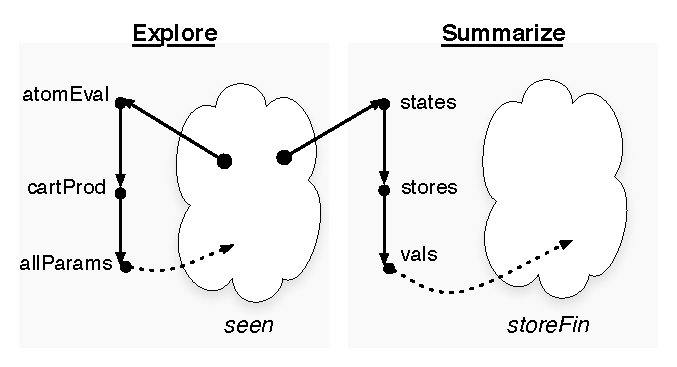
\includegraphics[width=3.1in]{chapter4/figures/DataFlowNet.pdf}
\end{center}
\vspace{-4mm}
  \caption{Simplified handler network for $k$-CFA.  Exploration and
    summarization processes are driven by the same LVar.  The triply-nested
    \lstinline{forEach} calls in \lstinline{summarize} become a chain of three handlers.}
\vspace{-4mm}
  \label{fig:dataflow}
\end{figure}


\paragraph{Flipping the switch}

%% \new{The LVish concurrent data structures have higher overhead if used only once
%%   without modification and copied repeatedly.
\new{The verbatim port uses LVars poorly: copying them repeatedly and discarding them
without modification.  This effect overwhelms the benefits of partial
deforestation and pipelining, and}
 the {\em verbatim} LVish port has a small performance overhead relative to the
 original.  But not for long!
% is a much easier starting point for overcoming the performance problems
% mentioned above.  
\new{The most clearly unnecessary operation in the verbatim port is in the
  \lstinline{next} function.}  Like the
pure code, it creates a fresh store to extend with new bindings as we take each
step through the state space graph:
\begin{lstlisting}
   store' <- IM.copy store 
\end{lstlisting}
Of course, a ``copy'' for an LVar is persistent: it is just a handler that
forces the copy to receive everything the original does.  But in LVish, it is
also trivial to {\em entangle} the parallel branches of the search, allowing them to
share information about bindings, simply by {\em not} creating a copy:
\begin{lstlisting}
   let store' = store 
\end{lstlisting}
This one-line change speeds up execution by up to $25\times$ on a single thread, and the
asynchronous, @ISet@-driven parallelism enables subsequent parallel speedup as well
(up to $202\times$ total improvement over the purely functional version).

Figure~\ref{fig:bench} shows performance data for the ``blur'' benchmark drawn
from a recent paper on $k$-CFA \cite{earl-might-icfp-2012}.  (We use $k=2$ for the
benchmarks in this section.)  In general, it proved difficult to generate
example inputs to $k$-CFA that took long enough to be candidates for parallel
speedup.  We were, however, able to ``scale up'' the blur benchmark by
replicating the code $N$ times, feeding one into the continuation argument for
the next.  Figure~\ref{fig:bench} also shows the results for one synthetic benchmark
that managed to negate the
benefits of our sharing approach, which is simply a long chain of $300$ ``not''
functions (using a CPS conversion of the Church encoding for booleans).  It has a small state space of large states with many
variables (600 states and 1211 variables).

%% Other simple attempts, however, to generate large synthetic
%% benchmarks simply wouldn't go slow enough. 

%%  (For example, we created a tree of
%% conditionals that converged very quickly).  


\paragraph{The role of lock-free data structures}
As part of our library, we provide lock-free implementations of
finite maps and sets based on concurrent skip lists~\cite{art}.\footnote{In fact,
  this project is the first to incorporate {\em any} lock-free data
  structures in Haskell, which required solving some unique problems
  pertaining to Haskell's laziness and the GHC compiler's
  assumptions regarding referential transparency.  But we lack the space to
  detail these improvements.}  We
also provide reference implementations that use a nondestructive
@Data.Set@ inside a mutable container.
% 
Our scalable implementation is not yet carefully optimized, and at one
and two cores, our lock-free $k$-CFA is $38\%$ to $43\%$ slower than the reference implementation on the ``blur'' benchmark.
% (/ 5.21 3.64) (/ 2.69 1.94)
%
But the effect of scalable data structures is quite visible on a 12-core
machine.\footnote{Intel Xeon 5660; full machine details available at \url{https://portal.futuregrid.org/hardware/delta}.}
Without them, ``blur'' (replicated $8\times$) stops scaling and begins
% and plateaus or 
slowing down slightly after four cores.  Even at four cores, variance is high in
the reference implementation (min/max $0.96$s / $1.71$s over 7 runs).  With
lock-free structures, by contrast, performance steadily improves to a speedup of
$8.14\times$ on 12 cores ($0.64$s at $67\%$ GC productivity).
Part of the benefit of LVish is to allow purely functional programs to
make use of lock-free structures, in much the same way that the \texttt{ST} monad allows
access to efficient in-place array computations.

\if 0 % sadly no space for this...
Finally, we note that other search processes can benefit from sharing
information asynchronously through a shared ``blackboard'', especially if doing
so is deterministic and easy to use, as it is with LVish.  Processes that
monotonically restrict (\eg, shrinking sets) the possibilities are also
candidates.  In the future, we plan to examine parallel logic programming in
this light.
\fi

% blurN_8 times, delta, median of 7 trials WITH -qa (which makes a difference):
% 1:  5.21  (92% productivity)
% 2:  2.69
% 4:  1.42  (3.66X speedup)   REALTIME 1.39 1.41 1.49
% 6:  1.06
% 8:  0.84
% 10: 0.75
% 12: 0.64  (67% productivity, 8.14X speedup)

%% pure-in-a-box version, min/med/max:
%% The variance is large.
% 1:  REALTIME 3.64 3.65 3.65
% 2:  REALTIME 1.92 1.94 1.95
% 4:  REALTIME 1.20 1.33 1.53
% 6:  REALTIME 1.14 1.57 1.69
% 8:  REALTIME 1.15 1.50 1.70
% 10: REALTIME 0.96 1.46 1.71
% 12: REALTIME 1.15 1.43 1.71

% (/ 3.65 1.43) 2.5x
% (/ 3.65 1.33) 2.7X

\begin{figure}  
\lk{TODO: Ryan, we should try to make this legible when printed black
  and white.}

%% This could be a bar-chart showing the 
%% parallel speedup for cfa-lvish-in place,
%% and having one "broken" bar with a 
%% number at the top for the slow original perf
\begin{center}
  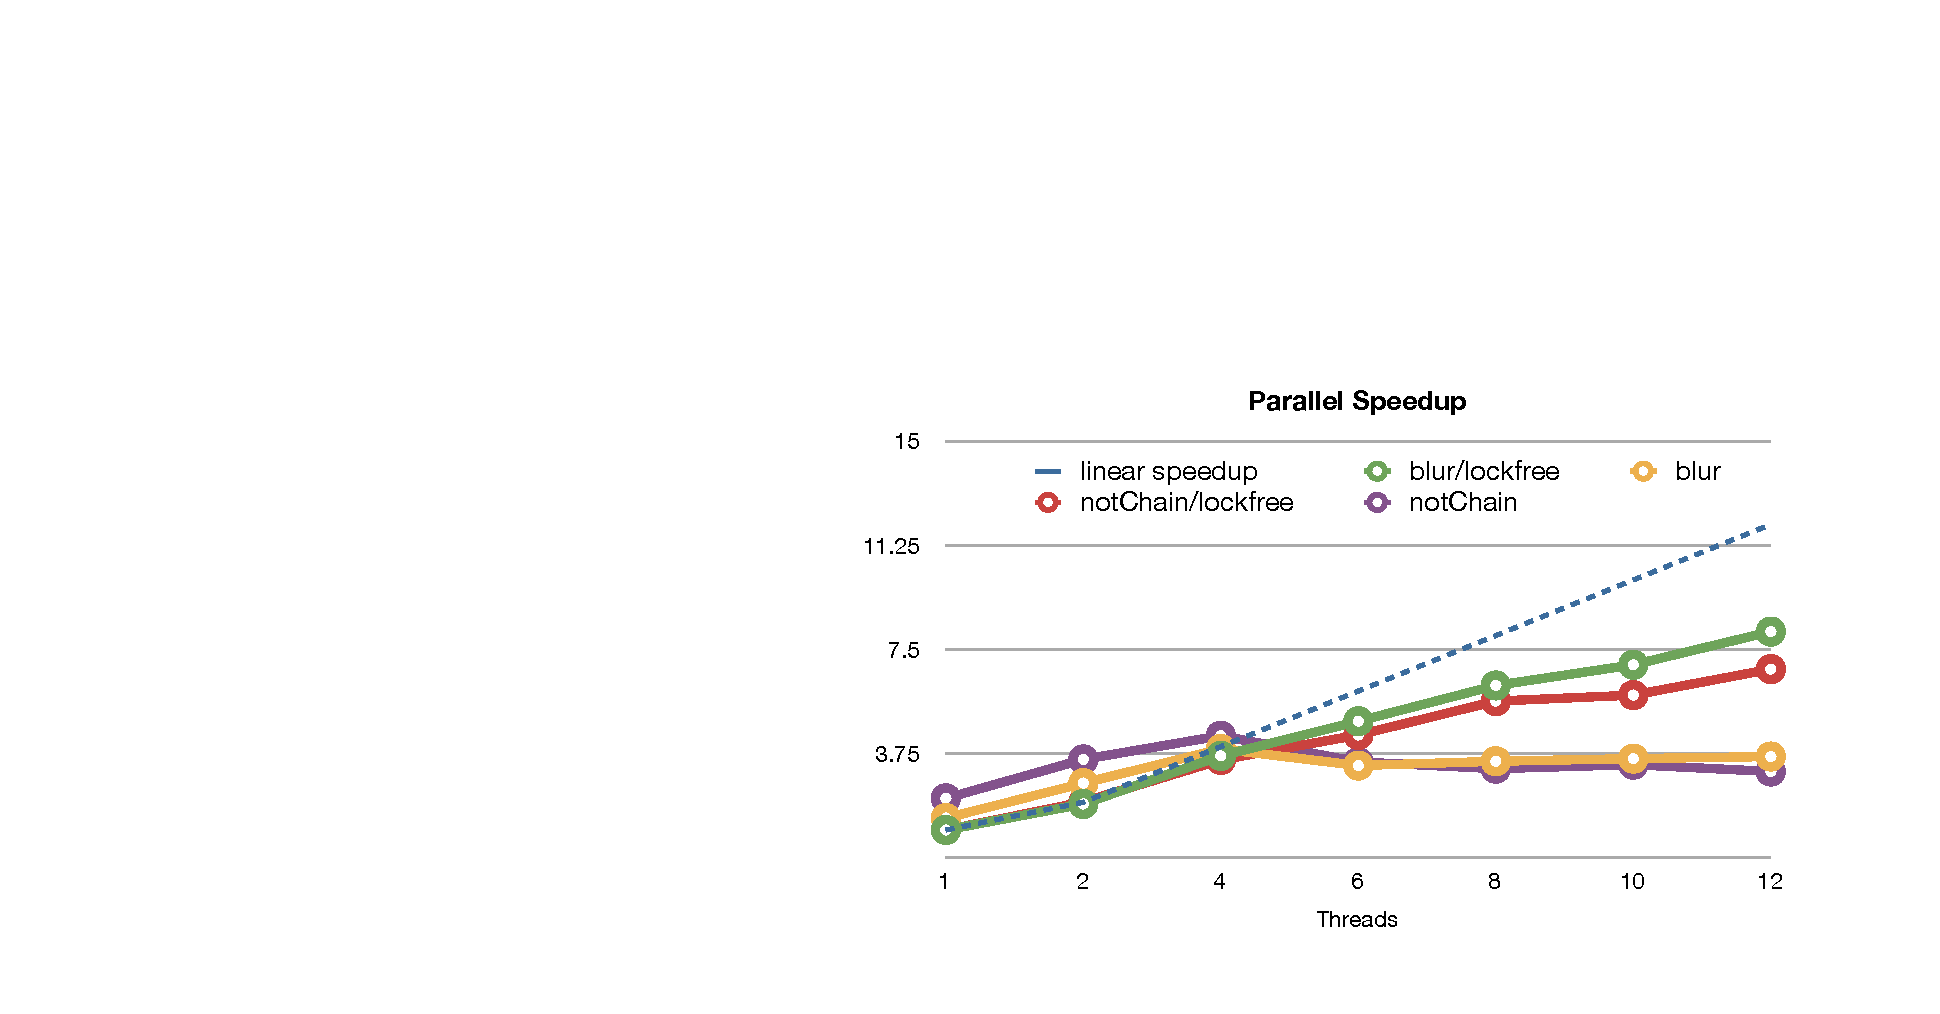
\includegraphics[width=3.3in]{chapter4/figures/CFA_speedups.pdf}
\end{center}
  \caption{Parallel speedup for the ``blur'' and ``notChain'' benchmarks.
    Speedup is normalized to the sequential times for the {\em lock-free}
    versions (5.21s and 9.83s, respectively).  
%
    The normalized speedups are remarkably consistent for the lock-free version
    between the two benchmarks.  But the relationship to the original, purely
    functional version is quite different: at 12 cores, the lock-free LVish
    version of ``blur'' is $202\times$ faster than the original, while ``notChain'' is only
    $1.6\times$ faster, 
    not gaining anything from sharing rather than copying stores
    due to a lack of fan-out in the state graph.
%% which we suspect is due to the lack of optimization in our
%%     skiplist implementation.
}
% \vspace{-4mm}
  \label{fig:bench}
\end{figure}



%% \begin{figure}  
%% \begin{verbatim}
%% .....................................
%%   NOT A LOT IN THIS ONE
%%   IT SHOULD PROBABLY GET MERGED INTO A TABLE
%% .....................................
%% \end{verbatim}
%%   \caption{A synthetic 2-CFA benchmark chaining three-hundred {\tt not} operations.}
%%   \label{fig:notchain}
%% \end{figure}


\TODO{Add benchmarks and case study from PLDI paper.}
